\section{Experimental Evaluation}\label{sec:eval}
%We have implemented each of the improvements. % we review in \autoref{subsec:improving-baseline}. 
\begin{figure}
  \centering
    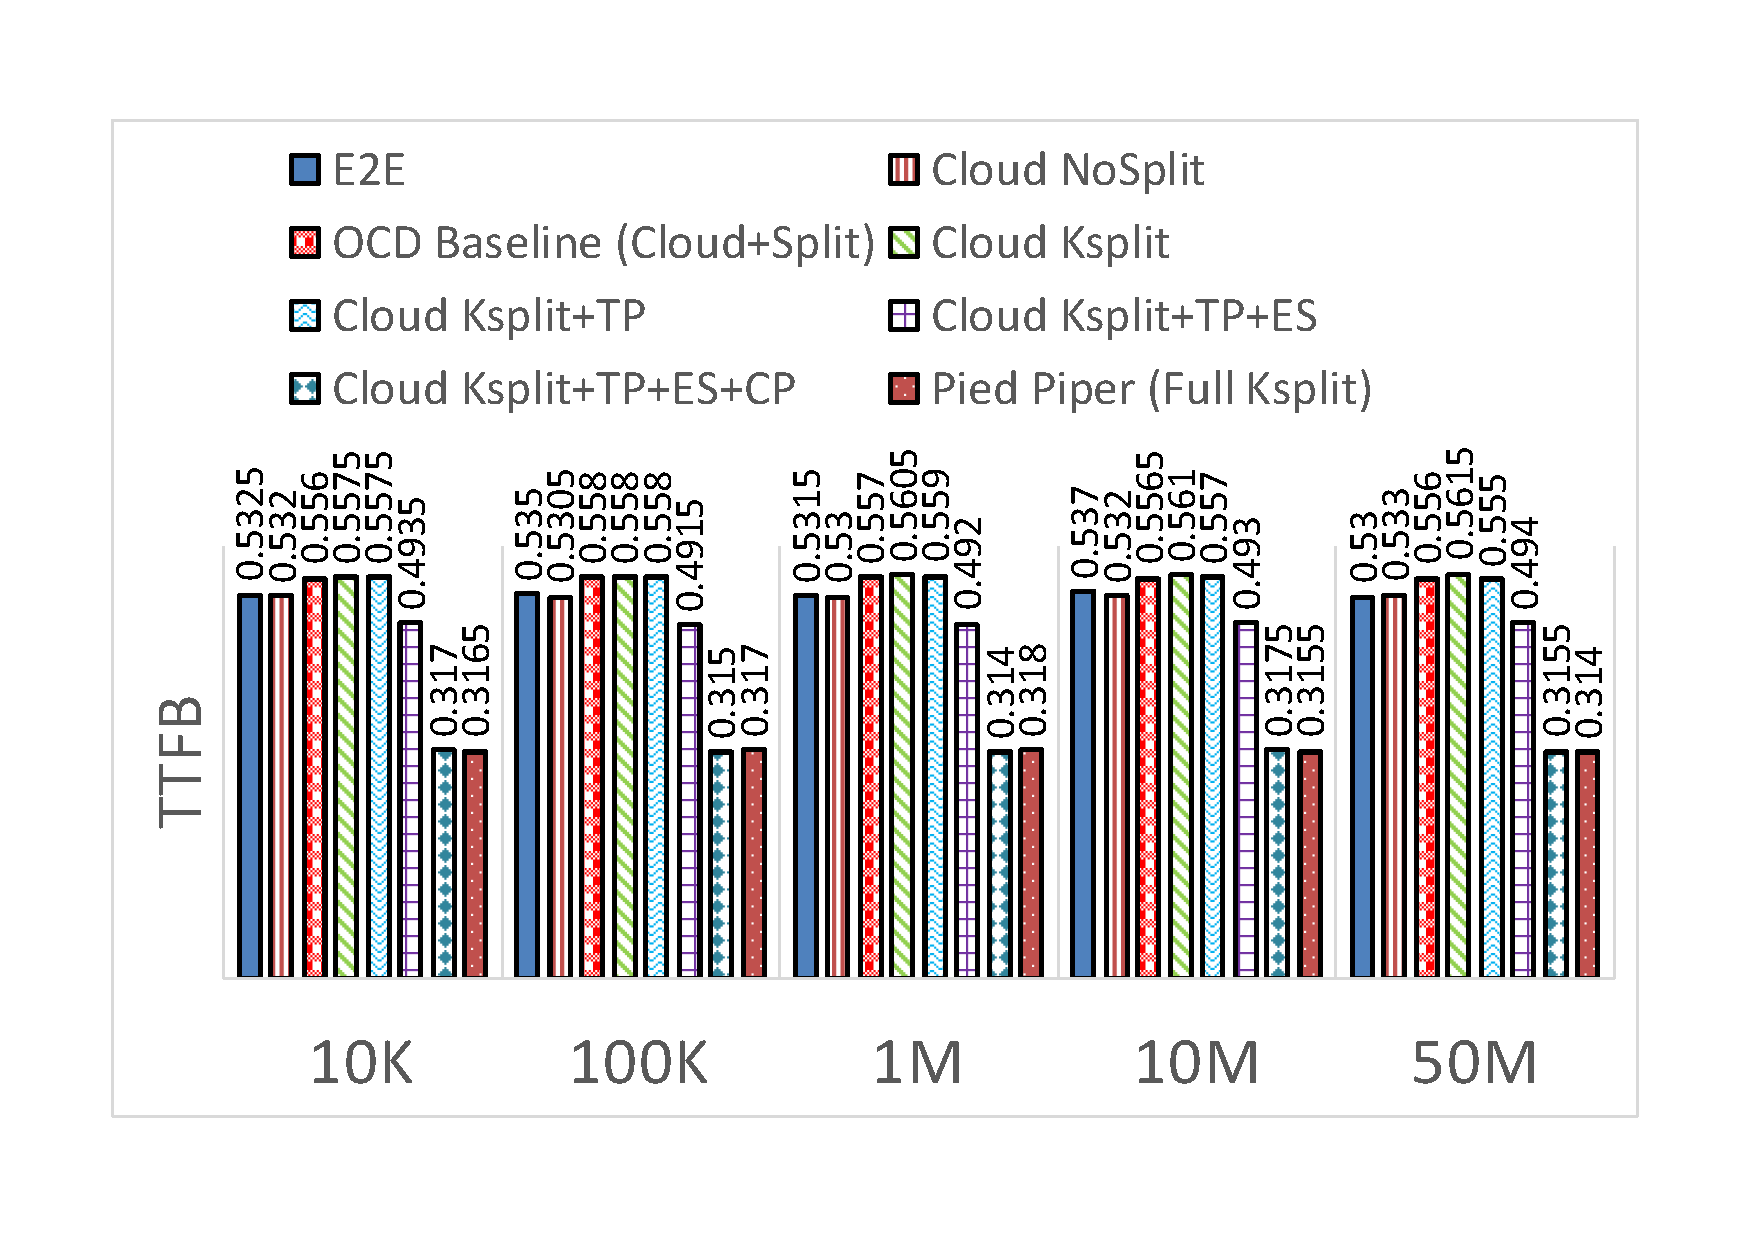
\includegraphics[width=\columnwidth,trim=20mm 25mm 20mm 22mm,clip]{figures/oursys-ttfb.pdf}
    \caption{Time-To-First-Byte (TTFB) in seconds. Median results of 50 runs.}%\AB{Come to think of it, all of these results are basically the same. The TTBF is not suppossed to change between different file sizes, and the results corroborate this. All in favor of just keeping one? pick your favorite :-)} 
    \label{fig:oursys-ttfb}
\end{figure}

\begin{figure}
  \centering
    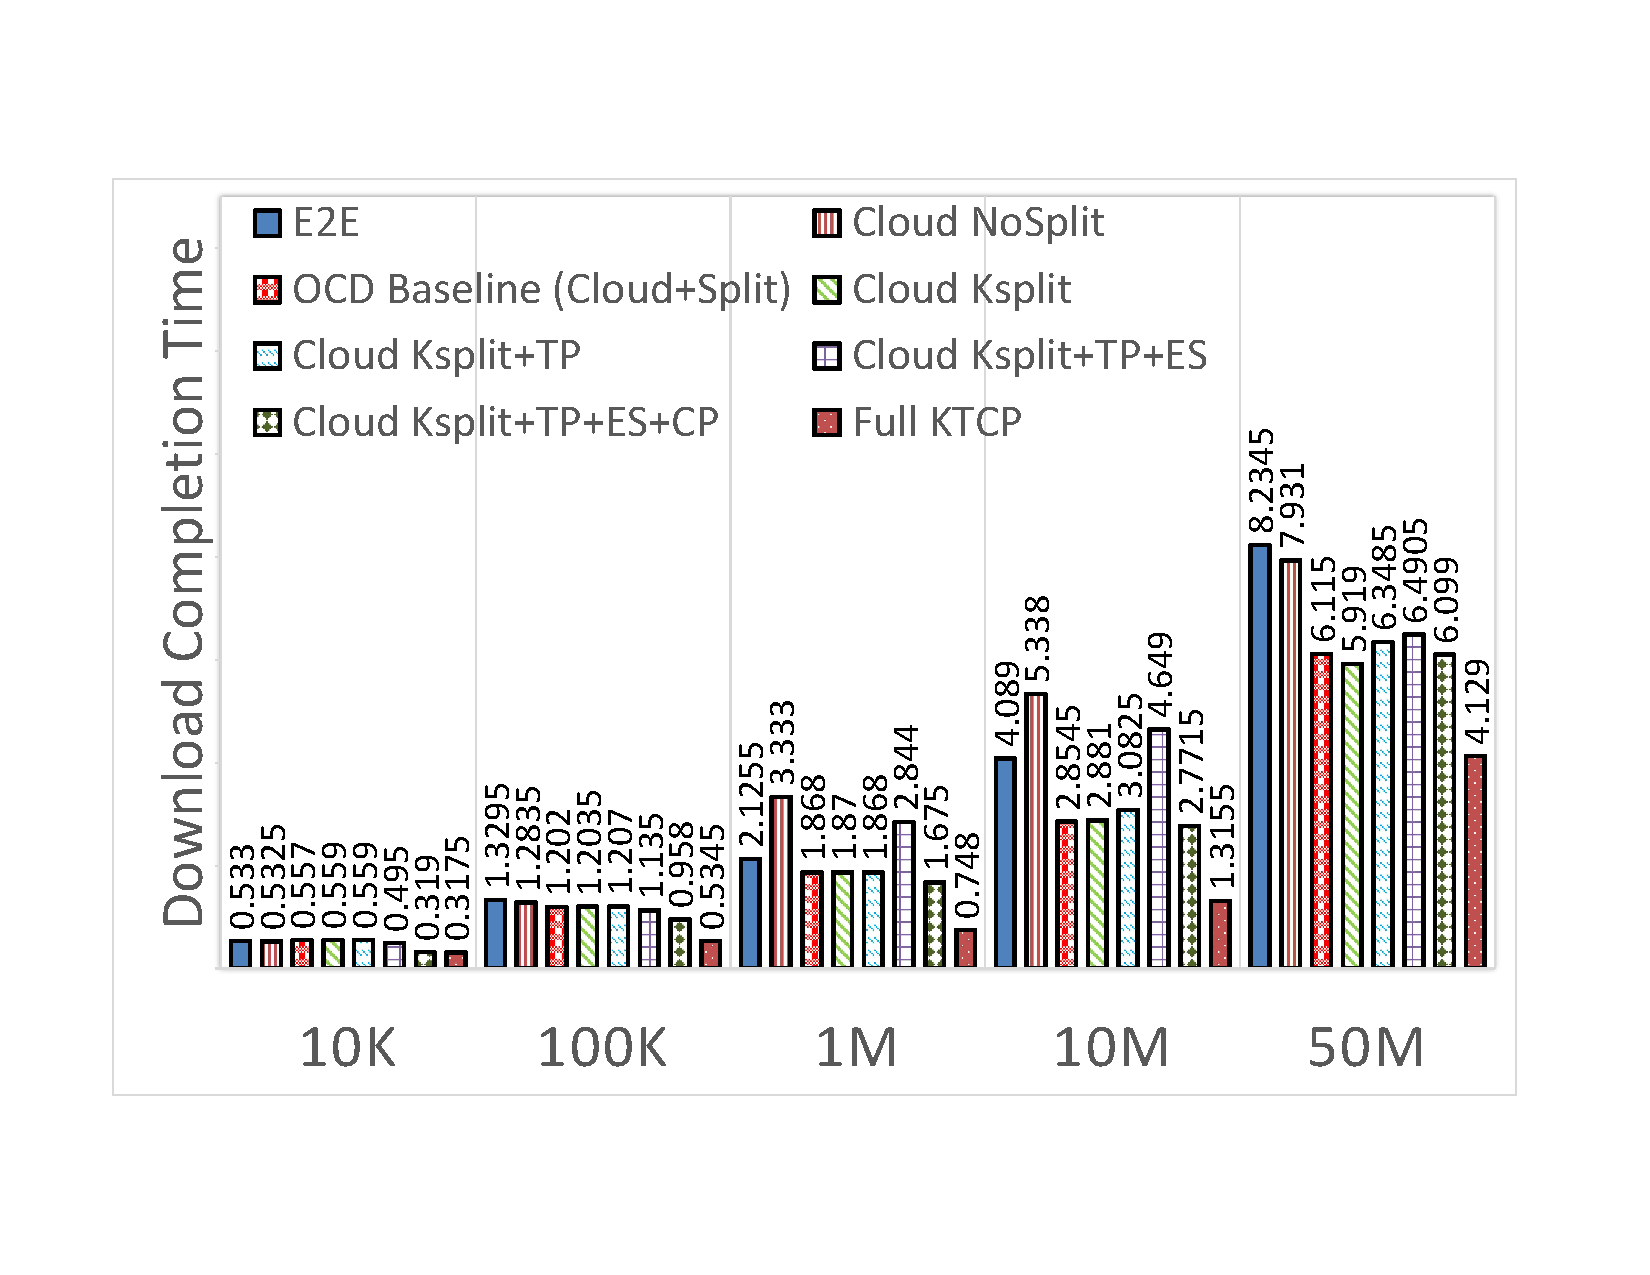
\includegraphics[width=\columnwidth,trim=20mm 25mm 20mm 23mm,clip]{figures/oursys-download.pdf}
    \caption{Download completion time in seconds. Median results of 50 runs.} 
    \label{fig:oursys-download}
\end{figure}

To evaluate the contribution of each of these improvements, we set up a server in Bangalore as a VM on a Digital Ocean infrastructure; and a client PC in San-Francisco, connected using a residential Internet service \footnote{The ISP is Comcast.}. Our relays are two VMs on GCP's public cloud: one in Mumbai, close to the server (\rs), and another (\rc)  in Oregon, near the client. Both VMs run on Ubuntu 17.04 and use small (n1-standard-1) machines with a single vCPU and $3.75$ GB memory. The client and server are Ubuntu 16.04 machines.

We set up an Apache web server on the Bangalore VM and evaluate the performance of each of the options by measuring both download times and time-to-first-byte (TTBF). We experiment with files of different sizes that the client is downloading from the server, using HTTP via the curl utility. The times reported in \autoref{fig:oursys-ttfb} and \autoref{fig:oursys-download}  are as returned by the curl utility.

The RTT  (as measured by ICMP) between the client and $\rc$ is $32.7$ms, between $\rc$ and $\rs$ is $215$ms, and between $\rs$ and the server is $26$ms.

We compare the performance of the following configurations: \begin{romanlist}
     \item simple End-to-End (\textit{e2e});
     \item routing through the cloud relays; using iptable's DNAT, without splitting the TCP flow (Cloud NoSplit);
     \item splitting the TCP flow using SSH's port forwarding feature (\textit{Baseline});
     \item TCP splitting using our \oursys kernel module, set up to use the improvements listed in \autoref{sec:approx}: thread pool only (\oursys+TP), thread pool and early-SYN (\oursys+TP+ES), a complete bundle of the three connection improvements including \reconn (\oursys+TP+ES+CP), and finally also configuring the intra-cloud TCP connection to use Turbo-Start (\textit{\oursys}).
\end{romanlist}

The benefit from the improvements is best observed by looking at the Time-To-First-Byte in \autoref{fig:oursys-ttfb}. We can see that the  TTFB and total download time of the basic \oursys coincide with those of the Baseline. Our basic kernel-based implementation performs at least as well as the well-established ssh utility. We also note that \oursys+TP does not improve the median performance by a noticeable amount. However, we have noticed throughout our testing that the thread pool improves the stability of our results.

For all file sizes we notice an improvement of $\approx60ms$ when using \oursys+TP+ES. This is in line with \autoref{fig:baseline}, as Early-SYN eliminates one RTT on the $(\mbox{client}\leftrightarrow\rc)$ and another RTT of the $(\rs\leftrightarrow\mbox{server})$. The amount of time reduced, according to our RTT measurements is supposed to be $59$ms, in line with our results. Adding \reconns to the mix should potentially reduce the TTFB by one RTT of the $(\rc\leftrightarrow\rs)$ leg. However, since the REQ cannot be forwarded with the SYN packet sent by the client (without any TCP extensions), we can only gain $215-33=182$ms. Indeed, the benefit of adding CP as evident in \autoref{fig:oursys-ttfb} is of $\approx 180$ms. The addition of Turbo-Start does not reduce the TTFB, as it only influences the way packets are sent after the first bytes. The contribution of Turbo-Start is clearly evident when considering the total download time (\autoref{fig:oursys-download}). We see considerable reduction of the file download time when using Turbo-Start for all file sizes, except that of 10 KB file. The default initial congestion window size for both Ubuntu 17.04 and 16.04 is 10 segments, so the entire file is sent in a single burst. Indeed, the results show that for 10 KB file the download completion time is about 1 ms after the first byte arrives. All other improvements contribute to the reduction of TTFB, and so reduce the total download time by roughly the same amount. This reduction is barely noticeable for large files, where the main benefits stem from splitting the TCP flow and using Turbo-Start.
In this experiment we notice that the best performing implementation improvement (\ie \oursys) outperforms e2e file transfer by up to 3 times! (depending on the file size).

%We also consider what benefit OCD can present to clients with limited memory, such as old PCs, small battery- and/or price-limited devices as well as other clients on the Internet which might advertise a limited receive window. Google noted in their QUIC paper \cite{quic} that 4.6\% of the clients downloading video from their servers (March 2016) had a limited receive window of 64KB. For large-RTT flows, this limited receive window directly limits the maximum throughput of a TCP flow. This is due to TCP's flow-control mechanism. OCD reduces the RTT of the first hop considerably,\footnote{compared to the original e2e RTT.} and thus potentially reaches a higher throughput with the same small receive window.
%we assumeme it can greatly improve the download speeds  for such clients. 
%To assess the benefits such clients might gain from using OCD, we rerun \oursys and K-Split+TP+ES+CP experiments and compare their performance when the client's receive socket buffer is limited to 64 KB. The results are presented in \autoref{fig:oursys-weak-client}. We see up to a $7.91\times$ speed up when using \oursys for clients with a limited receive buffer. For 10 KB files the improvement is much more modest, as the receive window is not the limiting factor. In this case, all the benefits are due to the TTFB reduction. 

%To summarize, we demonstrated in this section how we can, with some acceleration techniques within our kernel implementation of TCP split, improve download times of files  of all sizes, and also improve latencies by reducing TTFB.


%\begin{figure}
%  \centering
%    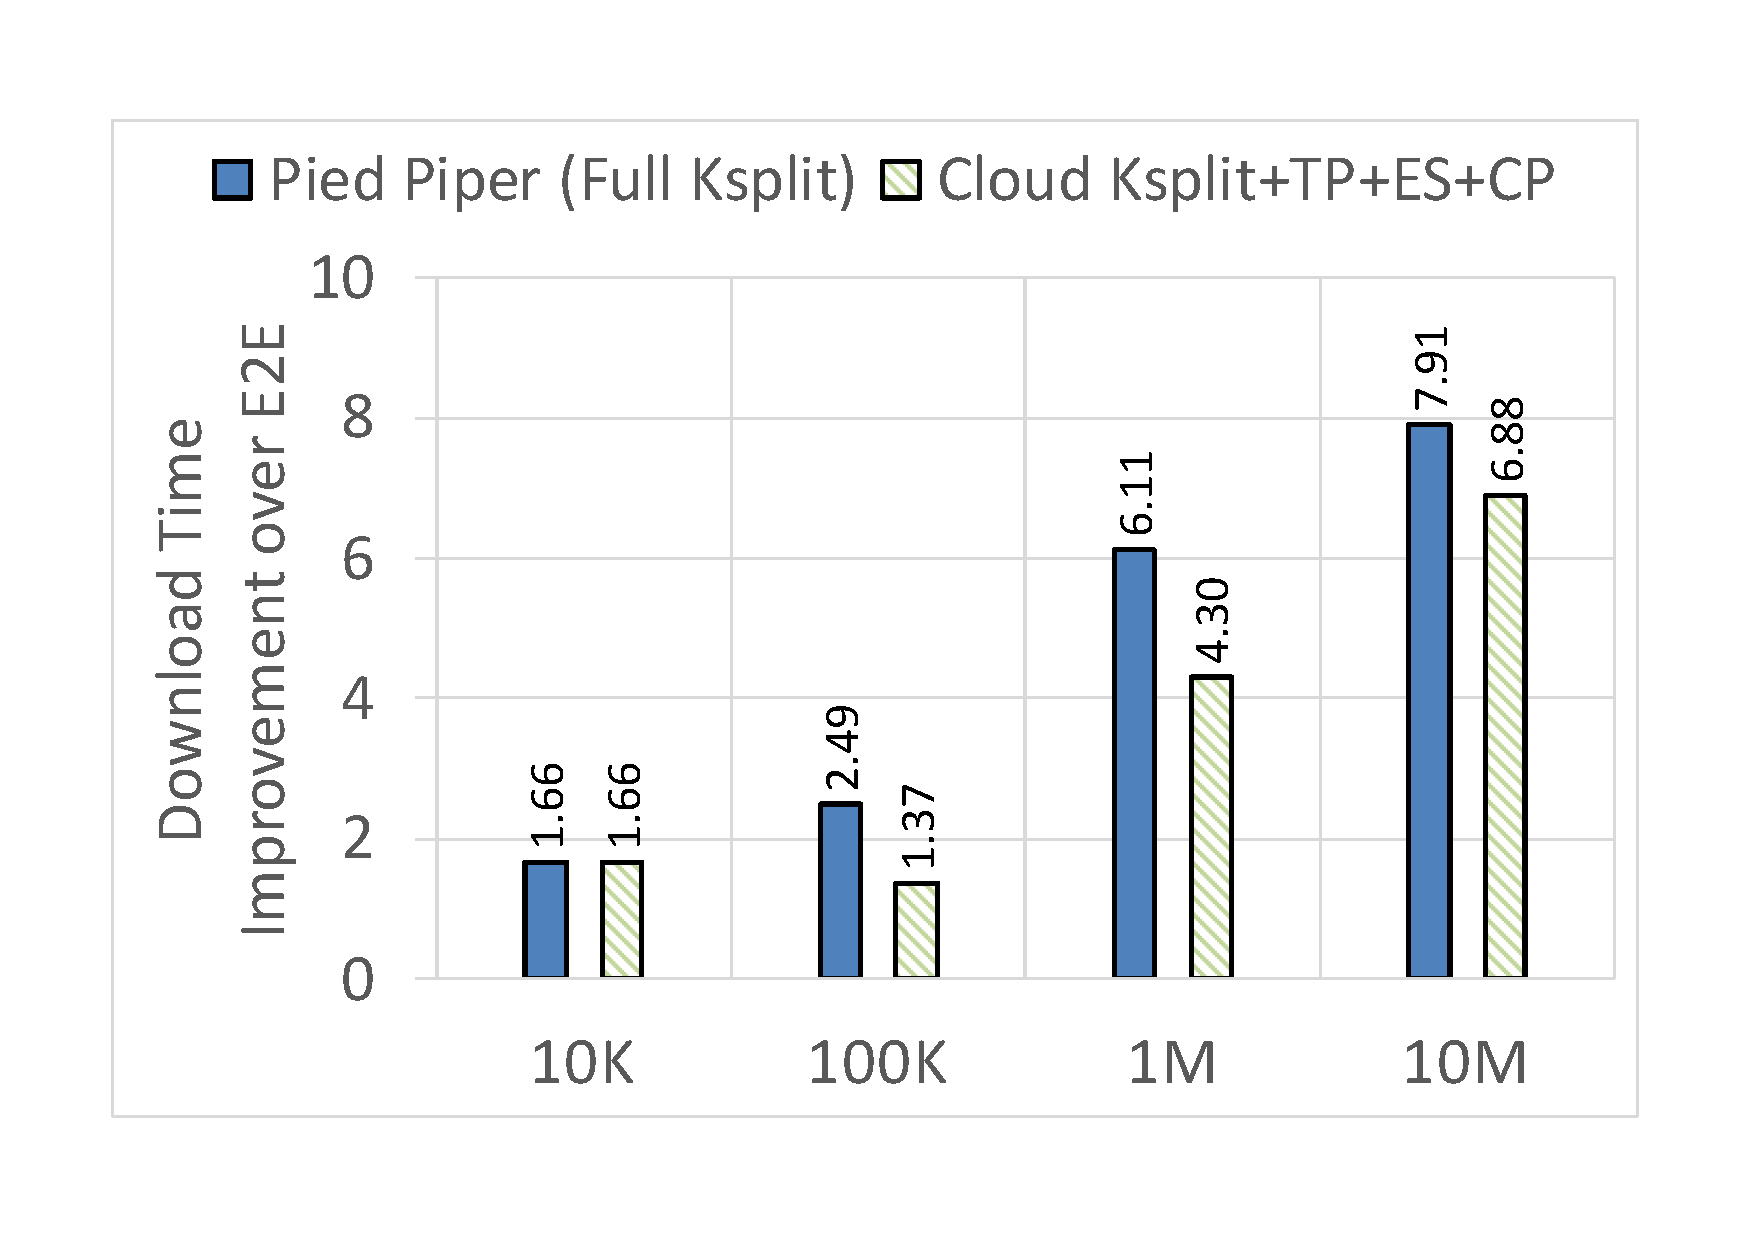
\includegraphics[width=\columnwidth,trim=20mm 25mm 25mm 25mm,clip]{figures/WeakClient-Improvement.pdf}
%    \caption{Improvement of \oursys performance over e2e in the case of a memory-limited client. Averaged results over 30 runs.} 
%    \label{fig:oursys-weak-client}
%\end{figure}

% \section{Routing Strategy}\label{sec:routing-strategy}

% \IK{Do we want to include the results here, or only mention strategies then have an experimental section?}

% 1 vs. 2 vs. 3 relays, intra-cloud vs. multiple clouds, ...


%\IK{Also need to check going through points outside the cloud: here are settings we mentioned:\\
%1. France-Switzerland-Prashanth(SF)-Israel(SF), or\\
%2. France-Switzerland-Amazon(SF)-Israel(SF), \ie half cloud}
